\documentclass[11pt,a4paper]{article}
\usepackage{graphicx}
\usepackage[parfill]{parskip}
\usepackage[table]{xcolor}
\usepackage{fullpage}
\usepackage{array}
\newcolumntype{L}{>{\centering\arraybackslash}m{0.18\textwidth}}
\newcommand{\highPrio}{\cellcolor{green}High}
\newcommand{\medPrio}{\cellcolor{orange}Medium}
\newcommand{\lowPrio}{\cellcolor{yellow}Low}
\newcommand{\vLowPrio}{\cellcolor{yellow!50}Very Low}
\title{CodeBuzz}
\author{Team Gocky \\
    Craig McLaughlin, 1002524M \\
    Gordon Reid, 1002536R}
\begin{document}

\maketitle

\newpage

\section*{Abstract}

This report documents the specification and design of CodeBuzz,
a web-application for posting code snippets. The aim of the application is
to facilitate programming language learning by exposing beginners to
example programs written by industry experts and academics, and to
aid reuse by providing a store of solutions to commonly recurring
problems in software engineering. 
\newpage

\tableofcontents
\newpage

\section{Introduction}

CodeBuzz is a code snippet oriented application that allows users to submit code
in a variety of programming languages. This code is categorised based on the
code's language, and function (e.g. sorting algorithm). This categorisation
will allow other users to search for code snippets (e.g. Python Bubble Sort)
and have returned to them a list of matching snippets. These can be ordered
by popularity or user rating.

When a user views a code snippet they have the option to copy the snippet into
their clipboard or comment and rate the snippet.

The application can be used by novice coders looking for examples of common
language functions and can be used by intermediate/expert programmers to supply
their own examples, and rate others. Academics may also find this of use as
it can provide a convenient source of example code (which may or may not be
good code, both useful in this context).

\section{Functionality}

The site will operate similar to any collaborative web-based application
where users of the site need not be registered in order to contribute
to the site content. The functionality is detailed in the lists below.

The following functionality is available to both registered and
non-registered users:

\begin{itemize}
\item Code snippets have their syntax highlighted.
\item Snippet hit rate/popularity.
\item Categorised code snippets by language and function.
\item Ability to search for code snippets based on language and
function.
\item Textual copy-to-clipboard.
\item Downloadable source code.
\item Links to other code snippets.
\end{itemize}

The following functionality is only available to registered users:
\label{sec:restrict}

\begin{itemize}
\item User can comment on the code snippets, e.g. reviewing the
correctness/usefulness of the code snippet.
\item User can rate a code snippet on a five star scale.
\item User profile which stores bookmarked snippets.
\item Social network integration.
\end{itemize}

\newpage

\section{Application Design Ideas}

\subsection{Wireframes}

Figure \ref{fig:anonsnippet} shows an anonymous snippet being posted by a
visitor to the website who has chosen not to log in. An example of the basic
layout and the syntax highlighting capabilities are shown in the figure.

Figure \ref{fig:joe} shows a logged in user posting a snippet. The user's
name is shown and there are also links to his profile, bookmarks, and other
user-specific data.

Figure \ref{fig:LoggedInViewJane} shows a user called Jane logged in and viewing
a snippet posted by an anonymous user. There is rating and comments section
with a text box for Jane to add in her own comment if she wishes. The page
scrolls as the comments are not necessarily immediately available above the
fold.

Figure \ref{fig:viewCategories} shows a user called Jane logged in and viewing
the snippet categories. Snippets fit into two categories: language, and type.
The view is identical if the user isn't logged in, with the obvious exception
of the upper bar. The upper bar would look like what was shown in Figure
\ref{fig:anonsnippet}.

\begin{figure}
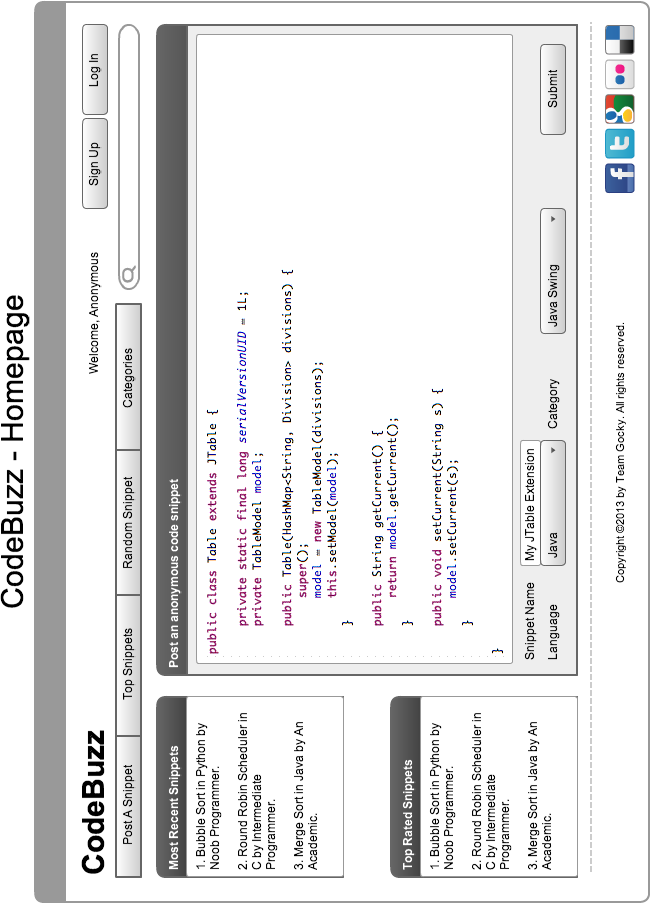
\includegraphics[width=\textwidth]{../imgs/homepageWireFrameGRHorz.png}
\caption{Anonymous snippet being posted.}
\label{fig:anonsnippet}
\end{figure}

\begin{figure}
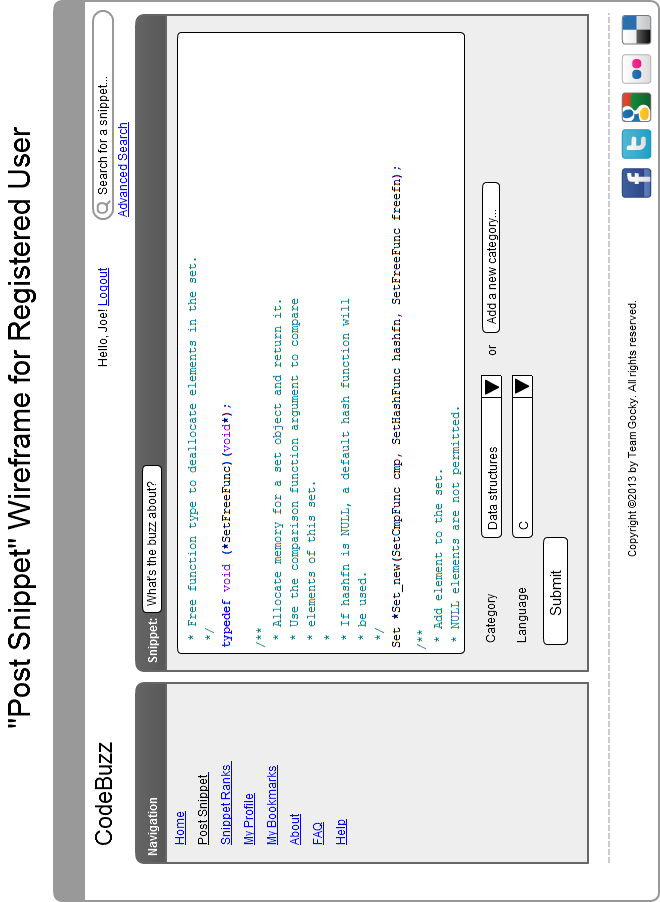
\includegraphics[width=\textwidth]{../imgs/CCodeSnippetHorz.png}
\caption{Joe's home screen with his code snippet}
\label{fig:joe}
\end{figure}

\begin{figure}
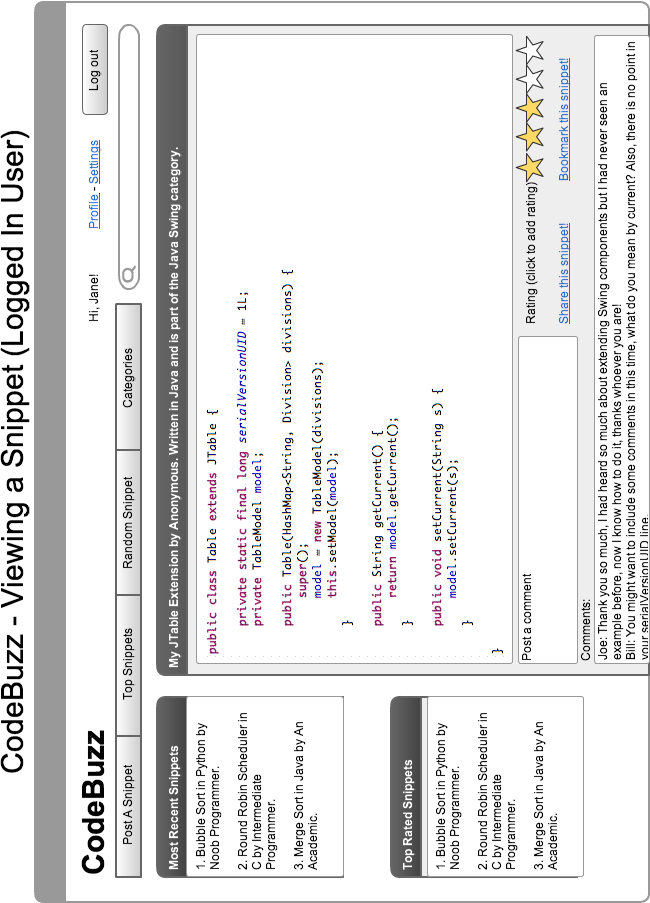
\includegraphics[width=\textwidth]{../imgs/LoggedInViewSnippetHorz.png}
\caption{Jane viewing a posted snippet.}
\label{fig:LoggedInViewJane}
\end{figure}

\begin{figure}
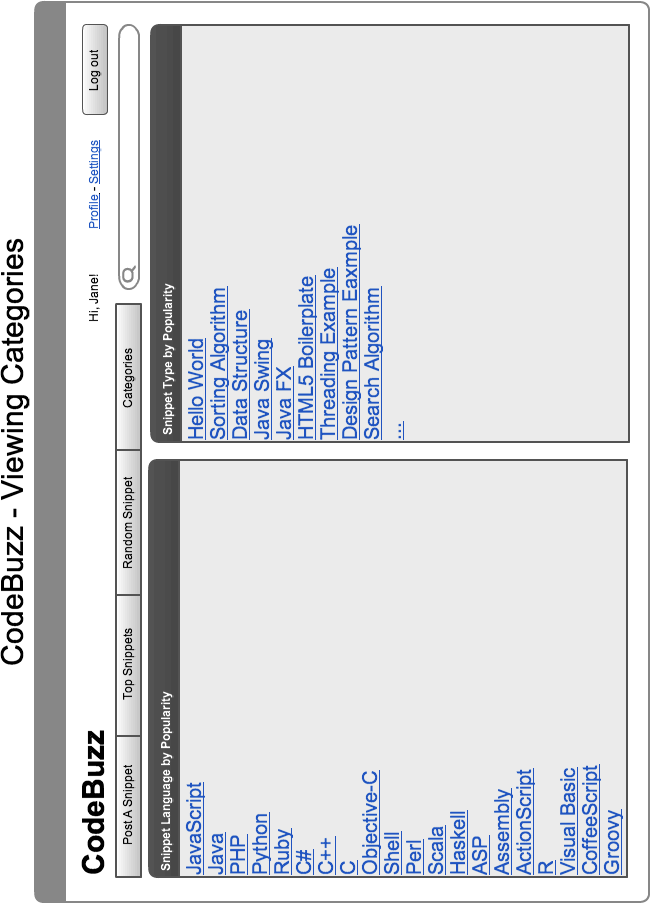
\includegraphics[width=\textwidth]{../imgs/viewingCategoriesHorz.png}
\caption{Jane looking at the categories of snippet.}
\label{fig:viewCategories}
\end{figure}

\subsection{Design Goals}

The number one design goal is to make the user interface minimalist
such that the user is not overwhelmed by the application. As can be
seen in the wire frames described above, the application will have a simple
home screen both for registered and non-registered users.

\subsection{A Walk through: Submit a code snippet in C}

A simple walk through for the user Jane entering her C code snippet as
shown in Figure~\ref{fig:joe} is given below:

\begin{enumerate}
\item Jane logs in using her user details.
\item Jane is presented with the home screen.
\item Jane selects the C programming language from the language drop-down
menu.
\item Jane proceeds to write her C code into the main window.
\item Jane selects the `Data Structures' category from the category
drop-down menu.
\item Jane is finished creating her code snippet and clicks the `Submit'
button.
\item Jane logs out.
\end{enumerate}

Note that the walk through above is applicable to a non-registered user
as well. For restrictions on non-registered users see
Section~\ref{sec:restrict}.

This walk through has highlighted a number of interactions between the
user and the application. It is important to note the order in which
the steps are carried out, particularly the selection of the
programming language and the entering of the code. The order is
important because the selection will dynamically set the syntax
highlighting mode in the application to the language specified.
The text that the user then enters is highlighted according to the
language selected. This highlighting is performed on-demand. % (!)
However, the application will not enforce this ordering on the user.

\newpage

\section{Personas}

\subsection{Barry: The Noob Programmer}
\label{sec:barry} 

Barry is sixteen, studying a computing based course and is looking to
learn a particular language. Barry's programming ability is, at best,
amateur. He relies heavily on introductory texts and Internet forums
since his school does not provide learning materials for the language
of interest.

\subsubsection{Goals}

\begin{itemize}
\item Finding code snippets to perform a specific programming task,
e.g. reading from a file.
\item Looking for code on a particular language.
\item To download/copy the code snippet for integration into their
program.
\item Comment on a snippet to ask questions if understanding is low.
\end{itemize}

\subsubsection{Behaviours}

\begin{itemize}
\item Curiosity towards others code for inspiration for their own code
development. Looking for ideas on, `How it's done', etcetera.
\item Impatient regarding the `slowness' of their learning, wanting to
get their application up and running as soon as possible. Quick and
dirty.
\end{itemize}

\subsubsection{Likes}

\begin{itemize}
\item Syntax-highlighted environments that help his inexperienced brain
comprehend what is going on.
\item When code works out of the box.
\item Easy-to-read code, using simple constructs and ideas so that it
is simple to digest.
\end{itemize}

\subsubsection{Dislikes}

\begin{itemize}
\item Being unable to find the desired code snippet, or one which is
too complex/advanced for their current abilities.
\item Being overwhelmed by large number of advanced search capabilities.
\end{itemize}

\newpage

\subsection{Bill: The Academic}

Dr Compton is a University Professor teaching software engineering at
one of the top universities in his country. He wishes to contribute
code to a publicly accessible forum for his research area to entice
people to join his research project entitled
\textit{Software Elasticity in Safety-Critical Systems}. He also wishes
to publish code for courses he teaches to promote a social coding
environment for use by his students. His aim is to get all his students
using CodeBuzz to submit coursework, share interesting code samples,
etc, instead of other social networking sites so they stop
wasting their lives having meaningless conversations about cats on
invisible bikes with strangers.

\subsubsection{Goals}

\begin{itemize}
\item Add source code simulation of software degradation and how it's
entropy decreases over time in a safety-critical environment.
\item Look for crowd-sourced examples of how, or how not to, code a certain
programming function for use in class.
\item Use as a platform for student-submitted code that can be peer-reviewed.
\item Looks to aid the learning of students and others in their programming.
\end{itemize}

\subsubsection{Behaviours}

\begin{itemize}
\item Comment/rate student-submitted code as part of the learning process.
\item Upload examples of standard/optimised solutions to coding problems.
\item Submits high quality code for re-use and to contribute to the Open
Source community.
\item Gives low ratings and disapproving comments to incorrect,
inefficient or ugly code snippets to discourage beginners from
adopting poor techniques or bad programming habits.
\end{itemize}

\subsubsection{Likes}

\begin{itemize}
\item The ability to review code snippets via comments and ratings.
\item Being able to provide sample high-quality, working solutions.
\end{itemize}

\subsubsection{Dislikes}

\begin{itemize}
\item Poor quality code being passed off as working.
\item Students not keeping up with work given.
\end{itemize}

\newpage

\subsection{Jane: Experienced Programmer}

Jane works in industry on medium-large commercial software projects. She has 
working knowledge of multiple programming languages and is well versed in 
different paradigms and making use of good software engineering concepts such as 
design patterns.

\subsubsection{Goals}

\begin{itemize}
\item Scout out potential future job candidates.
\item Suggest optimisations and changes to a user's submitted code.
\end{itemize}

\subsubsection{Behaviours}

\begin{itemize}
\item Becomes frustrated with other's mistakes however wishes to aid the
learning of individuals so they can become more proficient in programming.
\end{itemize}

\subsubsection{Likes}

\begin{itemize}
\item Seeing potential in other people for future job roles.
\end{itemize}

\subsubsection{Dislikes}

\begin{itemize}
\item Poor quality code being passed off as working.
\item Repeatedly being asked simple questions or seeing the same fundamental
errors.
\item Beginners that do not `R.T.F.M.'.
\end{itemize}

\newpage

\section{User Needs Matrix}

\begin{table}[h]
\begin{tabular}{*{6}{|L}|}
\hline
I want to... & Overall Priority & Barry & Bill & Jane\\
\hline
Search solution code & \highPrio & \highPrio & \medPrio & \lowPrio \\
\hline
Download code snippet & \highPrio & \highPrio & \medPrio & \lowPrio \\
\hline
Contribute quality code & \highPrio & \lowPrio & \highPrio & \highPrio \\
\hline
Rate a code snippet & \highPrio & \lowPrio & \highPrio & \medPrio \\
\hline
Comment on a snippet & \highPrio & \medPrio & \highPrio & \lowPrio \\
\hline
Bookmark a snippet & \medPrio & \medPrio & \highPrio & \medPrio \\
\hline
Submit code for review & \medPrio & \highPrio & \vLowPrio & \vLowPrio \\
\hline
Share code externally & \lowPrio & \medPrio & \vLowPrio & \vLowPrio \\
\hline
View highly rated code & \medPrio & \highPrio & \medPrio & \lowPrio \\
\hline
View code hit count & \lowPrio & \lowPrio & \vLowPrio & \vLowPrio \\
\hline
\end{tabular}
\end{table}

\end{document}  
